\subsubsection{Compito C4: Rinomina di un file}

Il compito C4 richiedeva all’utente di rinominare il documento ``Appunti\_Lezione.pdf'', precedentemente caricato all’interno della cartella principale, assegnandogli il nuovo nome ``Riassunto Primo Semestre''. L’obiettivo era valutare l’usabilità e la visibilità dei pulsanti dedicati alla gestione e modifica dei file personali, con particolare attenzione al flusso di rinomina.

\paragraph{Analisi delle prestazioni generali}

L'introduzione della versione post-riprogettazione (B) ha generato un progresso netto e confermato sul piano statistico nell'efficienza (Tabella~\ref{tab:6-c4-1}), ferma restando la riuscita dell'operazione per tutti i partecipanti in entrambe le modalità di test. In particolare, si osserva una contrazione solida e statisticamente rilevante del 40,33\% delle interazioni fisiche necessarie, con la media dei click che scende da 12,07 della versione originale a 7,20 della nuova interfaccia. Le restanti metriche prestazionali si configurano come semplici tendenze descrittive di miglioramento: sia il tempo medio di completamento sia la media degli errori registrano cali marginali e statisticamente non discriminanti, indicando andamenti favorevoli ma stabili sotto il profilo inferenziale.

Per quanto concerne la difficoltà percepita, la mediana registra una parziale oscillazione passando dal valore 1 al valore 2. Questo lieve incremento trova riscontro qualitativo nel trend descritto dai punteggi medi raffigurati nella Figura~\ref{fig:6-c4-1}, dove si osserva un aumento marginale da 1,80 a 1,87. La discrepanza tra il guadagno nel numero di click e la percezione soggettiva evidenzia la persistenza di piccoli attriti nell'interazione, riconducibili principalmente alla comprensibilità cognitiva del flusso.

\begin{figure}[H]
	\centering
	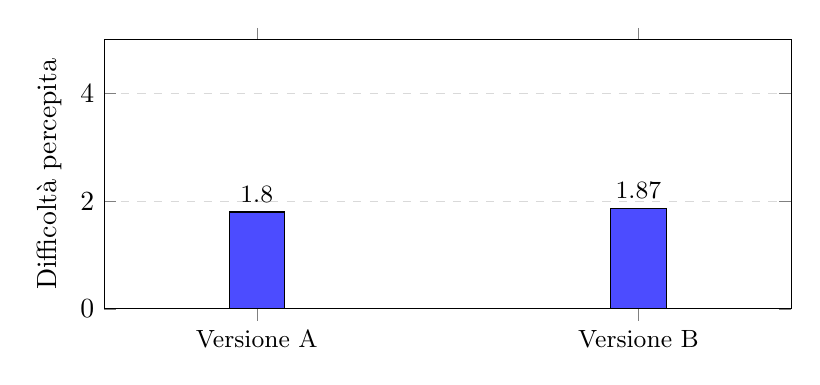
\begin{tikzpicture}
		\begin{axis}[
				ybar,
				bar width=20pt,
				width=0.85\textwidth,
				height=5cm,
				symbolic x coords={Versione A, Versione B},
				xtick=data,
				x tick label style={font=\small},
				ylabel={Difficoltà percepita},
				ymin=0, ymax=5,
				ymajorgrids=true,
				grid style={dashed, gray!30},
				enlarge x limits=0.4,
				nodes near coords,
				every node near coord/.style={font=\small, color=black},
			]
			\addplot+[
				ybar,
				fill=blue!70,
				draw=black
			] coordinates {
					(Versione A,1.80)
					(Versione B,1.87)
				};
		\end{axis}
	\end{tikzpicture}
	\caption{Confronto della difficoltà percepita tra Versione A e Versione B per C4.}
	\label{fig:6-c4-1}
\end{figure}

\begin{table}[H]
	\centering
	\footnotesize
	\renewcommand{\arraystretch}{1.2}
	\caption{Metriche prestazionali globali aggregate per il compito C4.}
	\label{tab:6-c4-1}
	\begin{tabular}{|>{\raggedright\arraybackslash}p{2.2cm}|>{\centering\arraybackslash}p{1.5cm}|>{\centering\arraybackslash}p{1.5cm}|>{\centering\arraybackslash}p{1.5cm}|>{\centering\arraybackslash}p{1.5cm}|>{\centering\arraybackslash}p{1.8cm}|>{\centering\arraybackslash}p{1.6cm}|}
		\hline
		\rowcolor{gray!30}
		\textbf{C4}           & \multicolumn{2}{c|}{\textbf{Versione A}} & \multicolumn{2}{c|}{\textbf{Versione B}} & \textbf{Variazione \%} & \textbf{Rilevanza}                                            \\ \hline
		\textit{Success Rate} & \multicolumn{2}{c|}{100,00\%}            & \multicolumn{2}{c|}{100,00\%}            & \textbf{Invariato}     &                                                               \\ \hline
		\rowcolor{gray!30}
		                      & \textbf{Media}                           & \textbf{DEV.ST}                          & \textbf{Media}         & \textbf{DEV.ST}    & \multicolumn{2}{c|}{}                    \\ \hline
		\textit{Errori}       & 0,60                                     & 1,12122                                  & 0,533                  & 0,83381            & \textbf{-11,11\%}     & \pvalue{0,82750} \\ \hline
		\textit{Tempo}        & 0.56.40                                  & 0,02057                                  & 0.51.04                & 0,01302            & \textbf{-9,88\%}      & \pvalue{0,48119} \\ \hline
		\textit{Click}        & 12,07                                    & 5,33809                                  & 7,20                   & 2,88345            & \textbf{-40,33\%}     & \pvalue{0,00486} \\ \hline
		\rowcolor{gray!30}
		                      & \multicolumn{2}{c|}{\textbf{Mediana}}    & \multicolumn{2}{c|}{\textbf{Mediana}}    & \multicolumn{2}{c|}{}                                                                  \\ \hline
		\textit{Difficoltà}   & \multicolumn{2}{c|}{1}                   & \multicolumn{2}{c|}{2}                   & \multicolumn{2}{c|}{}                                                                  \\ \hline
	\end{tabular}
\end{table}

La marcata diminuzione del numero di click riflette una maggiore efficacia del percorso d'azione riprogettato. Tuttavia, la percezione di una difficoltà lievemente maggiore evidenzia come la semplificazione delle operazioni sia stata in parte controbilanciata da incertezze qualitative nell'interazione.

\paragraph{Analisi qualitativa: commenti e osservazioni degli utenti}

L’incremento della difficoltà percepita, nonostante il miglioramento delle metriche di efficienza, trova riscontro nelle osservazioni raccolte. Nella versione riprogettata (B), l’ottimizzazione del percorso non sempre è risultata coerente con il modello mentale degli utenti. In particolare, sono emerse le seguenti criticità:

\begin{itemize}
	\item \textbf{Assenza di un’azione esplicita di rinomina}: diversi utenti si aspettavano la presenza di un comando dedicato ``Rinomina''. L’utilizzo di un comando più generico (es. ``Modifica'') ha introdotto incertezza sull’esito dell’azione.

	\item \textbf{Mancanza di pre-compilazione del campo}: il campo di input si presentava vuoto al momento dell’apertura del form, senza evidenziare il nome corrente del file pronto per la modifica. Questa scelta ha violato le aspettative degli utenti, generando un immediato attrito cognitivo (\textit{Gulf of Execution}). I dati mostrano come il vantaggio derivante dalla riduzione dei click (da 10 a 7) venga compensato dallo sforzo necessario per reinserire manualmente il testo, determinando un lieve incremento della difficoltà percepita.

	\item \textbf{Comportamento non immediato}: alcuni utenti hanno inizialmente tentato di modificare il nome direttamente dalla vista di anteprima del file, interpretando tale area come editabile. L’assenza di questa funzionalità ha generato passaggi a vuoto e ritorni alla schermata precedente.
\end{itemize}

Per la versione originale (A), le criticità risultano meno strutturali e principalmente legate alla visiblità dei menu contestuali. In particolare, alcuni utenti hanno avuto difficoltà nell’individuare le opzioni di gestione del file, con conseguente incremento del numero di interazioni necessarie.

\paragraph{Valutazione dell’effetto di apprendimento}

La scomposizione dei risultati in base all'ordine di presentazione dei sistemi (Tabella~\ref{tab:6-c4-2}) evidenzia l'impatto positivo dell'apprendimento soprattutto nel gruppo A--B. Per questa sequenza di test, la metrica sui click medi registra un miglioramento solido del 44,23\%, scendendo da 11,56 a 6,44. I restanti indicatori prestazionali per lo stesso gruppo, comprese la media dei tempi di esecuzione e la media degli errori, evidenziano semplici tendenze descrittive di contrazione che non assumono rilevanza statistica. Nel gruppo B--A, gli andamenti positivi registrati per tutte le metriche prestazionali — comprese le riduzioni medie nei tempi e negli errori a favore della seconda prova, a fronte di un aumento medio dei click — non assumono rilevanza statistica e sono da interpretare come semplici trend descrittivi legati alla familiarizzazione con il task.

\begin{table}[H]
	\centering
	\footnotesize
	\renewcommand{\arraystretch}{1.2}
	\caption{Confronto delle metriche prestazionali in funzione dell'ordine di esecuzione per il compito C4.}
	\label{tab:6-c4-2}
	\begin{tabular}{|>{\raggedright\arraybackslash}p{2.2cm}|>{\centering\arraybackslash}p{1.0cm}|>{\centering\arraybackslash}p{1.0cm}|>{\centering\arraybackslash}p{1.8cm}|>{\centering\arraybackslash}p{1.6cm}|>{\centering\arraybackslash}p{1.0cm}|>{\centering\arraybackslash}p{1.0cm}|>{\centering\arraybackslash}p{1.8cm}|>{\centering\arraybackslash}p{1.6cm}|}
		\hline
		\rowcolor{gray!30}
		\textbf{Metrica}              & \multicolumn{4}{c|}{\textbf{Ordine A--B}} & \multicolumn{4}{c|}{\textbf{Ordine B--A}}                                                                                                                       \\ \cline{2-9}
		\rowcolor{gray!30}
		                              & \textbf{A}                                & \textbf{B}                                & \textbf{Variazione \%} & \textbf{Rilevanza} & \textbf{B} & \textbf{A} & \textbf{Variazione \%} & \textbf{Rilevanza} \\ \hline
		\textit{Tempo (Media)}        & 1.01.07                                   & 0.48.13                                   & \textbf{-21,09\%}      & \pvalue{0,22931}   & 0.55.20    & 0.50.00    & \textbf{-9,64\%}       & \pvalue{0,59421}   \\ \hline
		\textit{Errori (Media)}       & 0,89                                      & 0,556                                     & \textbf{-37,50\%}      & \pvalue{0,52374}   & 0,500      & 0,17       & \textbf{-66,67\%}      & \pvalue{0,36322}   \\ \hline
		\textit{Click (Media)}        & 11,56                                     & 6,44                                      & \textbf{-44,23\%}      & \pvalue{0,03409}   & 8,33       & 12,83      & \textbf{54,00\%}       & \pvalue{0,06165}   \\ \hline
		\textit{Difficoltà (Mediana)} & 1                                         & 1                                         &                        & \pvalue{}          & 2          & 1,5        &                        & \pvalue{}          \\ \hline
	\end{tabular}
\end{table}

Coerentemente con questo scenario, la valutazione soggettiva della difficoltà mostra una notevole stabilità. Sotto il profilo della mediana, il punteggio si attesta saldamente a 1 per entrambe le sessioni nel gruppo A--B. Le medie grafiche (Figura~\ref{fig:6-c4-2}) mostrano una lieve fluttuazione (da 1,78 della versione A a 1,89 della versione B), da interpretare come semplice trend descrittivo legato a un piccolo attrito transitorio nell'inserimento manuale del nome nel form vuoto della versione B. Nel gruppo B--A, la mediana sperimenta una parziale fluttuazione non determinante passando da 2 per la versione B a 1,5 per la versione A, supportata sul piano grafico da una media rimasta perfettamente invariata a 1,83 in entrambe le prove. Questo conferma che l'esperienza pregressa attenua le differenze percepite tra le due soluzioni.

\begin{figure}[H]
	\centering
	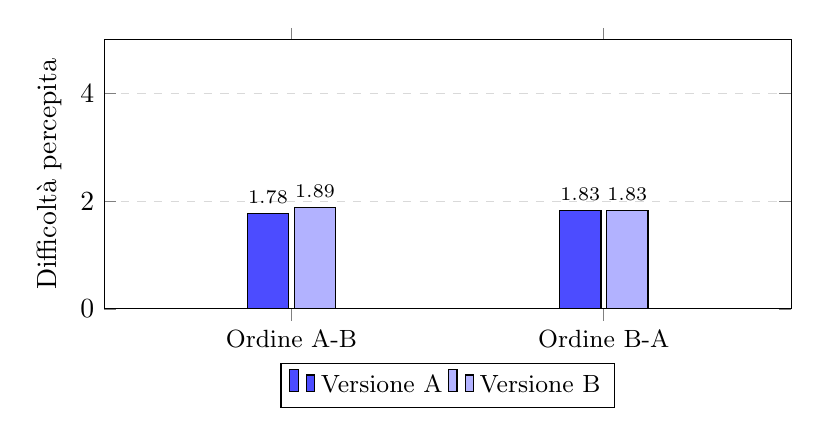
\begin{tikzpicture}
		\begin{axis}[
				ybar,
				bar width=15pt,
				width=0.85\textwidth,
				height=5cm,
				symbolic x coords={Ordine A-B, Ordine B-A},
				xtick=data,
				x tick label style={font=\small},
				ylabel={Difficoltà percepita},
				ymin=0, ymax=5,
				ymajorgrids=true,
				grid style={dashed, gray!30},
				enlarge x limits=0.6,
				legend style={at={(0.5,-0.2)}, anchor=north, legend columns=-1, font=\small},
				nodes near coords,
				every node near coord/.append style={font=\scriptsize, color=black},
			]
			\addplot+[
				fill=blue!70,
				draw=black
			] coordinates {
					(Ordine A-B,1.78)
					(Ordine B-A,1.83)
				};
			\addplot+[
				fill=blue!30,
				draw=black
			] coordinates {
					(Ordine A-B,1.89)
					(Ordine B-A,1.83)
				};
			\legend{Versione A, Versione B}
		\end{axis}
	\end{tikzpicture}
	\caption{Confronto della difficoltà percepita tra Versione A e Versione B per C4 in base all'ordine di esecuzione.}
	\label{fig:6-c4-2}
\end{figure}
